\documentclass[a4paper]{article}

\usepackage[T2A]{fontenc}
\usepackage[russian]{babel}
\usepackage{graphicx}
\usepackage{float}
\usepackage{hyperref}
\usepackage{amsmath, amssymb}
\usepackage{caption}
\usepackage{geometry}
\usepackage{pdfpages}
\geometry{top=2cm,bottom=2cm,left=2cm,right=2cm}

\newcommand{\minus}{\scalebox{0.75}[1.0]{$-$}}




\begin{document}

\begin{center}
\textsc{Санкт-Петербургский национальный исследовательский институт информационных технологий, механики и оптики\\[3mm]
Физический факультет} \\[3mm]

\end{center}
\vspace{5mm}
\line(1,0){\textwidth}
\begin{center}
\textbf{ЛАБОРАТОРНАЯ РАБОТА №1.13\\}
\textbf{"Изучение прецессии гироскопа"}
\end{center}
\vspace{2mm}
\line(1,0){\textwidth}
\vspace{5mm}
\begin{minipage}{0.4\textwidth}
    Группа: Z3144 \\
    Студент: Евгений Турчанин\\
    \vspace{1mm}
\end{minipage}
\hfill
\vspace{1mm}
\line(1,0){\textwidth}



\section{\textbf{Цели работы}}
\begin{enumerate}
\item Наблюдение прецессии гироскопа.
\item Экспериментальное подтверждение линейно зависимости периода прецессии гироскопа от частоты вращения гироскопа вокруг оси симметрии.
\item Экспериментальное определение момента инерции гироскопа
\end{enumerate}



\section{\textbf{Задачи}}
\begin{enumerate}
\item Измерить период прецессии гироскопа.
\item Измерить частоту вращения гироскопа вокруг своей оси.
\item Рассчитать момент инерции гироскопа относительно оси вращения используя данные полученные в ходе экперимента. Сравнить полученный результат с моментом инерции гироскопа, рассчитанным теоретически.
\end{enumerate}

\section{\textbf{Теория}}

Рассмотрим гироскоп закреплённый в точке совпадающей с центром масс так, что ось гироскопа, лежащая в горизонтальной
плоскости, может свободно поворачиваться в любом направлении. Пусть угловая скорость $\omega$ совпадает по направлению с осью вращение гироскопа, т.е. полный момент импульса:
\begin{equation}
\mathbf{M} = \mathbf{I} \omega
\end{equation}

где $I$ – момент инерции гироскопа относительно оси вращения,
совпадающей с одной из главных центральных осей. Пусть к оси
гироскопа приложена некоторая постоянная внешняя сила $F$, как
это показано на (рис. 1), т.е. перпендикулярно оси гироскопа.

\begin{figure}[H]
\begin{center}
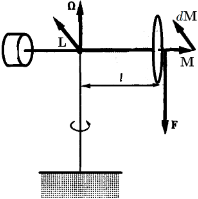
\includegraphics[width=0.3\textwidth]{pick_1.png}
\end{center}
\end{figure}

На ось гироскопа действует момент внешних сил $L$, по модулю равный:
\begin{equation}
L=Fl
\end{equation}

где $l$ – плечё силы $F$. Из уравнения моментов можно определить
направление вращения оси гироскопа:
\begin{equation}
    d \mathbf{M}=\mathbf{L} d t
\end{equation}
которая вращается с некоторой постоянной угловой скоростью $\Omega$,
называемой угловой скоростью прецессии, вокруг вертикальной
оси, проходящей через точку опоры гироскопа. Получим формулу, связывающую угловую скорость прецессии с угловой скоростью вращения гироскопа.\\
Пусть $d \varphi$ – угол на который поворачивается ось гироскопа вокруг вертикальной оси за время $d t$, тогда по определению:

\begin{equation}
    \Omega = \frac{\varphi}{d t}
\end{equation}
Модуль изменения момента импульс при этом можно записать
как,
\begin{equation}
    d M = M d \varphi
\end{equation}
с учётом формул (1), (2), (3), (4), (5) получим, что:
\begin{equation}
\Omega = \frac{Fl}{I\omega}
\end{equation}

т.о. зависимость угловой скорости прецессии от угловой скорости вращения гироскопа является обратно пропорциональной. Поскольку на эксперименте, чаще всего удобнее измерять период
нутации, а не угловую скорость, то формулу (7) удобно переписать в виде:
\begin{equation}
    T'=\dfrac{2\pi}{Fl}I\omega
\end{equation}
где $T'$ – период прецессии.


\section{\textbf{Данные}}

\begin{figure}[H]
\begin{center}
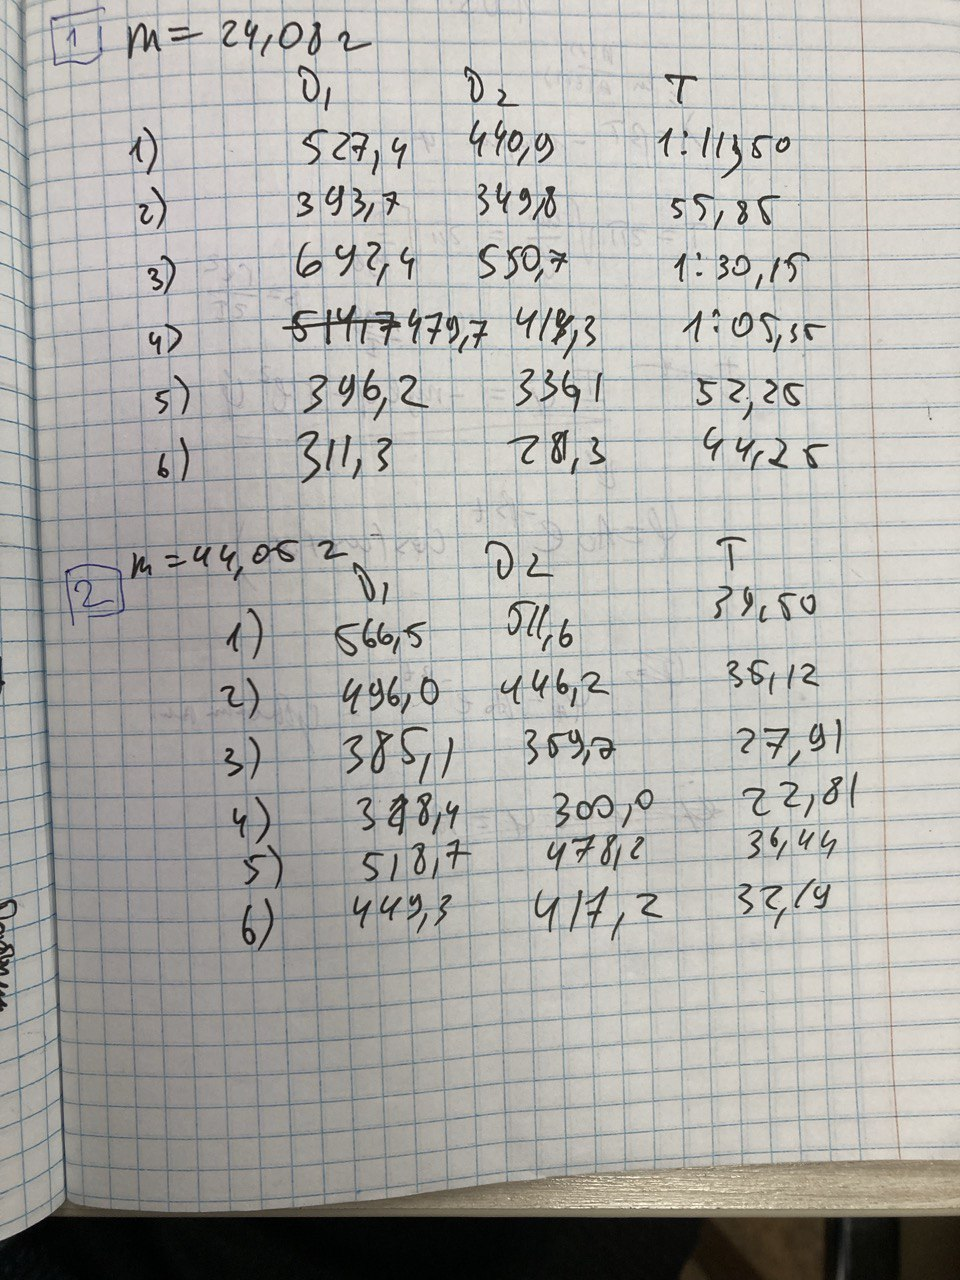
\includegraphics[width=0.3\textwidth]{pick_2.png}
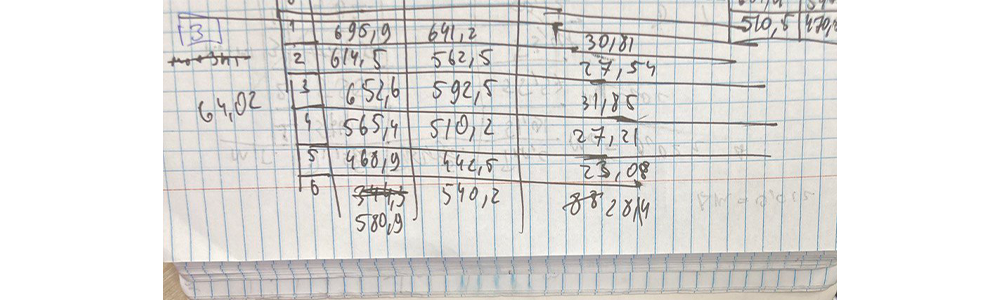
\includegraphics[width=0.5\textwidth]{pick_3.png}
\end{center}
\end{figure}


\section{\textbf{Результаты}}

С помощью питона обрабатываем данные и получаем следующие результаты:


\begin{figure}[H]
\begin{center}
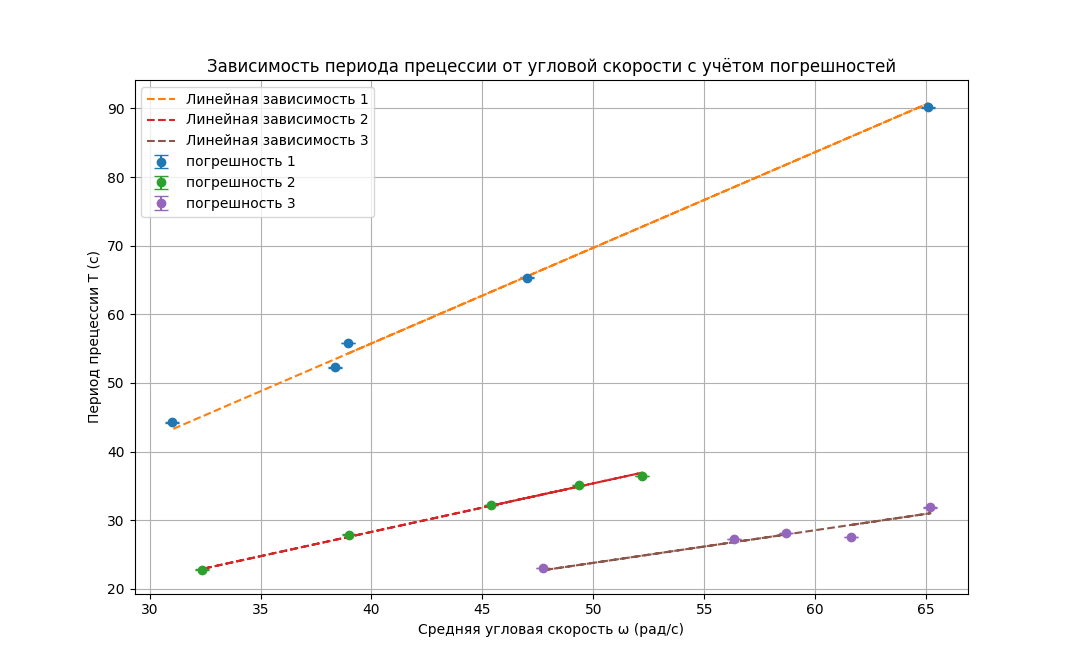
\includegraphics[width=0.3\textwidth]{pick_4.png}
\end{center}
\end{figure}



\end{document}
